\section{tree\_map\_for\_sequence} \label{sec-treemapseq}

This tools allows you to locate a certain sequence in a Newick tree. This
tool creates a \emph{map} file that you can use in conjunction with the
Newick utilities \cite{newick_tools} published by the University of Geneva, in
order to highlight clusters in different colors that contain such a certain
sequence.

\subsection{Usage}

The \emph{tree\_map\_for\_sequence} tool can be used as outlined
in the following:
\lstset{language=bash,
  caption={Calling the \emph{tree\_map\_for\_sequence} tool},
  label=lst-treemapseq-call}
\begin{lstlisting}
tree_map_for_sequence [fasta-ds] [fasta-seq] [color] [split-sets] > [map]
\end{lstlisting}
with the arguments:
\begin{enumerate}
  \item \emph{fasta-ds} A FASTA file containing the full dataset of
    that has been used to perform an adaptive clustering run, for instance,
    with the
    tools shown in section \ref{sec-adaptive-clust}.
  \item \emph{fasta-seq} A FASTA file containing the single sequence
    to be highlighted in a Newick tree by using this tool in conjunction
    with the Newick utilities.
  \item \emph{color} A string defining the color to use to mark
    clusters that contain the sequence in question. The color has to
    be expressed in a Cascade Style Sheet (CSS) compatible way. Hence,
    simple color expressions such as red, green and blue should
    work. In general it is preferred to use colors in the format
    \#RRGGBB where lead by a hash three hexadecimal numbers define the
    color values for red, green and blue. In order to
    get an orange color you may use, \#FF8800 which corresponds to
    full red, half green and no blue intensity. 
  \item \emph{split-sets} All the binary clusterings that are building the
    tree and that are used running the
    \emph{split\_sets\_to\_newick} tool, outlined in section
    \ref{sec-ssnewick}, in order to generate the
    dendogram that the Newick tools will
    use in the final tree visualization.
  \item \emph{map}
    The resulting \emph{map} file that can be used together with the
    Newick utilities to create a tree where all clusters containing
    a specific sequence are colored.
\end{enumerate}

\subsection{Example}
\lstset{language=bash,
  caption={Example of the \emph{tree\_map\_for\_sequence} tool},
  label=lst-treemapseq-example}
\begin{lstlisting}
tree_map_for_sequence test.fasta seq.fasta '#FF0000' /tmp/s* > tree.map
\end{lstlisting}
In this example we generate a map file \emph{tree.map} to color all
clusters that contain the sequence contained in \emph{seq.fasta} red in a
tree that we create using the Newick utilities. The tree was built from
the complete dataset of sequences found in \emph{test.fasta}. The
binary \emph{split-sets} that build the different layers of the tree
are found at \emph{/tmp/sX} where $X$ is the number of each layer. As
with all the previous tools the wild card selection should work
perfectly. To better illustrate the usage of the tool we show in the
following listing how this tool is used together with the the
\emph{split\_sets\_to\_newick} tool
described in section \ref{sec-ssnewick}, and the Newick utilities
\cite{newick_tools} by the university of Geneva:
\lstset{language=bash,
  caption={Further example of the \emph{tree\_map\_for\_sequence} tool},
  label=lst-treemapseq-example-extended}
\begin{lstlisting}
split_sets_to_newick 0 test.fasta 0 /tmp/s* > tree.dnd
tree_map_for_sequence test.fasta seq.fasta '#FF0000' /tmp/s* > tree.map
nw_display -w 600 -rs -i 'opacity:0' -b 'opacity:0' -l 'opacity:0' \
  -c tree.map tree.dnd > tree.svg
\end{lstlisting}
where \emph{tree.dnd} is the Newick file that corresponds to the \emph{map}
\emph{tree.map} that we generate with the tool outlined in this
section. The \emph{nw\_display} from the Newick utilities
\cite{newick_tools} creates a (Scalable Vector Graphics) SVG
image of our tree without annotations and a
width of 600 points in a radial fashion. It uses the aforementioned \emph{map}
to color clusters that contain the sequence to be highlighted red in the tree.
An example tree generated like this is shown in figure \ref{fig-treemapseq}.

\begin{figure}
  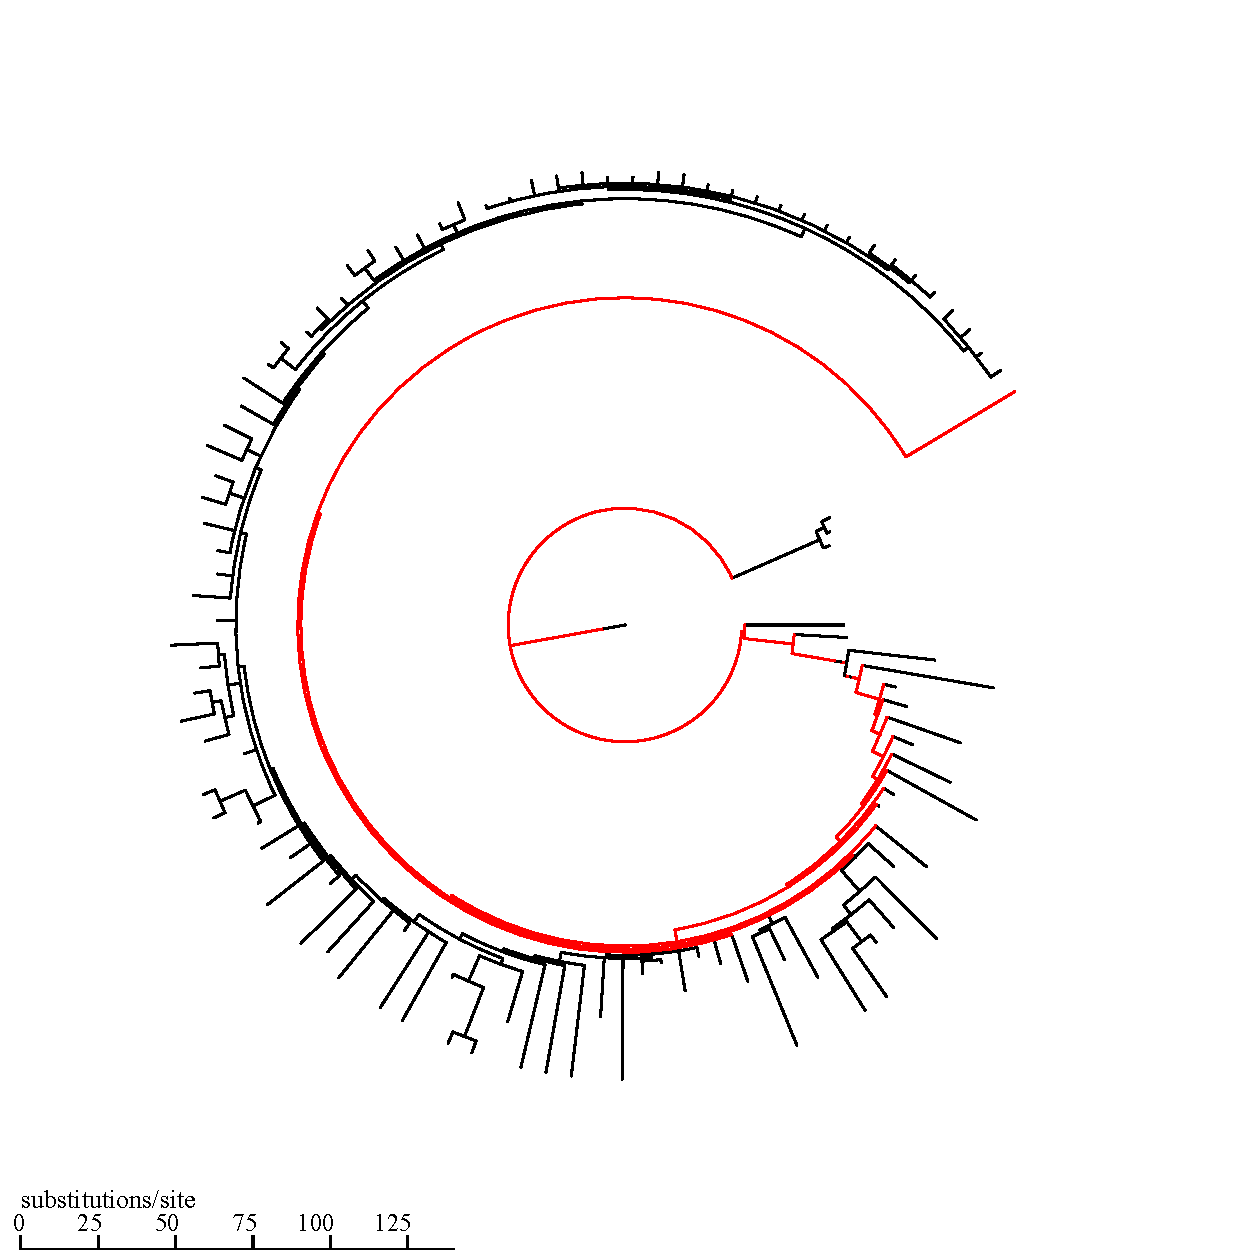
\includegraphics[scale=0.7]{tree-stroke.pdf}
  \caption{An example of a tree that outlines with a red line the
    location of a certain sequence. The commands to create such a tree
    are outlined in listing
    \ref{lst-treemapseq-example-extended}. The substitutions/site
    scale automatically generated by the Newick utilities
    \cite{newick_tools} and can be ignored.}
  \label{fig-treemapseq}
\end{figure}

\subsection{Implementation}
The \emph{tree\_map\_for\_sequence} tool is implemented in \newline
\emph{tree\_map\_for\_sequence.c}.

